\documentclass{article}
\usepackage[utf8]{inputenc}

\title{Test history project}
\author{paulo.reis }
\date{December 2018}

\usepackage{natbib}
\usepackage{graphicx}

\begin{document}

\maketitle

\section{Introduction}
There is a theory which states that if ever anyone discovers exactly what the Universe is for and why it is here, it will instantly disappear and be replaced by something even more bizarre and inexplicable.
There is another theory which states that this has already happened.

Lorem ipsum dolor sit amet, consectetur adipisicing elit, sed do eiusmod tempor incididunt ut labore et dolore magna aliqua. Ut enim ad minim veniam, quis nostrud exercitation ullamco laboris nisi ut  ex ea commodo consequat. Duis aute irure dolor in reprehenderit in voluptate velit esse cillum dolore eu fugiat nulla pariatur. Excepteur sint occaecat cupidatat non proident, sunt in culpa qui officia deserunt mollit anim id est laborum.

Lorem ipsum dolor sit amet, consectetur adipisicing elit, sed do eiusmod tempor incididunt ut labore et dolore magna aliqua. Ut enim ad minim veniam, quis nostrud exercitation ullamco laboris nisi ut aliquip ex ea commodo consequat. Duis aute irure dolor in reprehenderit in voluptate velit esse cillum dolore eu fugiat nulla pariatur. Excepteur sint occaecat cupidatat non proident, sunt in culpa qui officia deserunt mollit anim id est laborum.
\begin{figure}[h!]
\centering
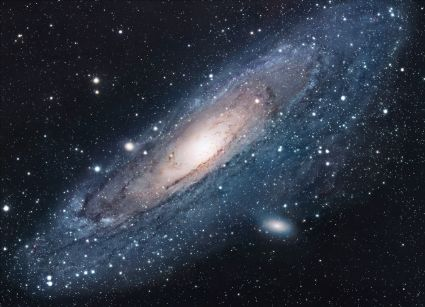
\includegraphics[scale=1.7]{universe}
\caption{The Universe}
\label{fig:universe}
\end{figure}

\section{Conclusion}
``I always thought something was fundamentally wrong with the universe'' \citep{adams1995hitchhiker}

\bibliographystyle{plain}
\bibliography{references}
\end{document}
